\section{Tiny DiT Validation}

We further test trend stability on a second, lightweight backbone using a Tiny DiT-style \texttt{Transformer2DModel}. This validation is designed as a controlled cross-backbone check, not a large-scale DiT benchmark.

\begin{table}[t]
  \centering
  \caption{Tiny DiT validation (10 epochs, ranks 4/8/16).}
  \label{tab:tiny_dit}
  \small
  \begin{tabular}{rrrrrrr}
    \toprule
    Rank & Trainable & Trainable(\%) & Runtime(s) & Peak MB & Final Loss & FID \\
    \midrule
    4  & 16384 & 1.5269 & 549 & 1753.54 & 0.1435 & 383.2438 \\
    8  & 32768 & 3.0078 & 545 & 1761.75 & 0.1425 & 387.8070 \\
    16 & 65536 & 5.8400 & 545 & 1778.18 & 0.1347 & 402.0335 \\
    \bottomrule
  \end{tabular}
\end{table}

In Tiny DiT validation, rank 4 again performs best and rank 8 remains competitive, while rank 16 is clearly worse in FID under the same budget. Figure~\ref{fig:ddpm_vs_tiny} compares DDPM and Tiny DiT trends for ranks 4/8/16.

\begin{figure}[t]
  \centering
  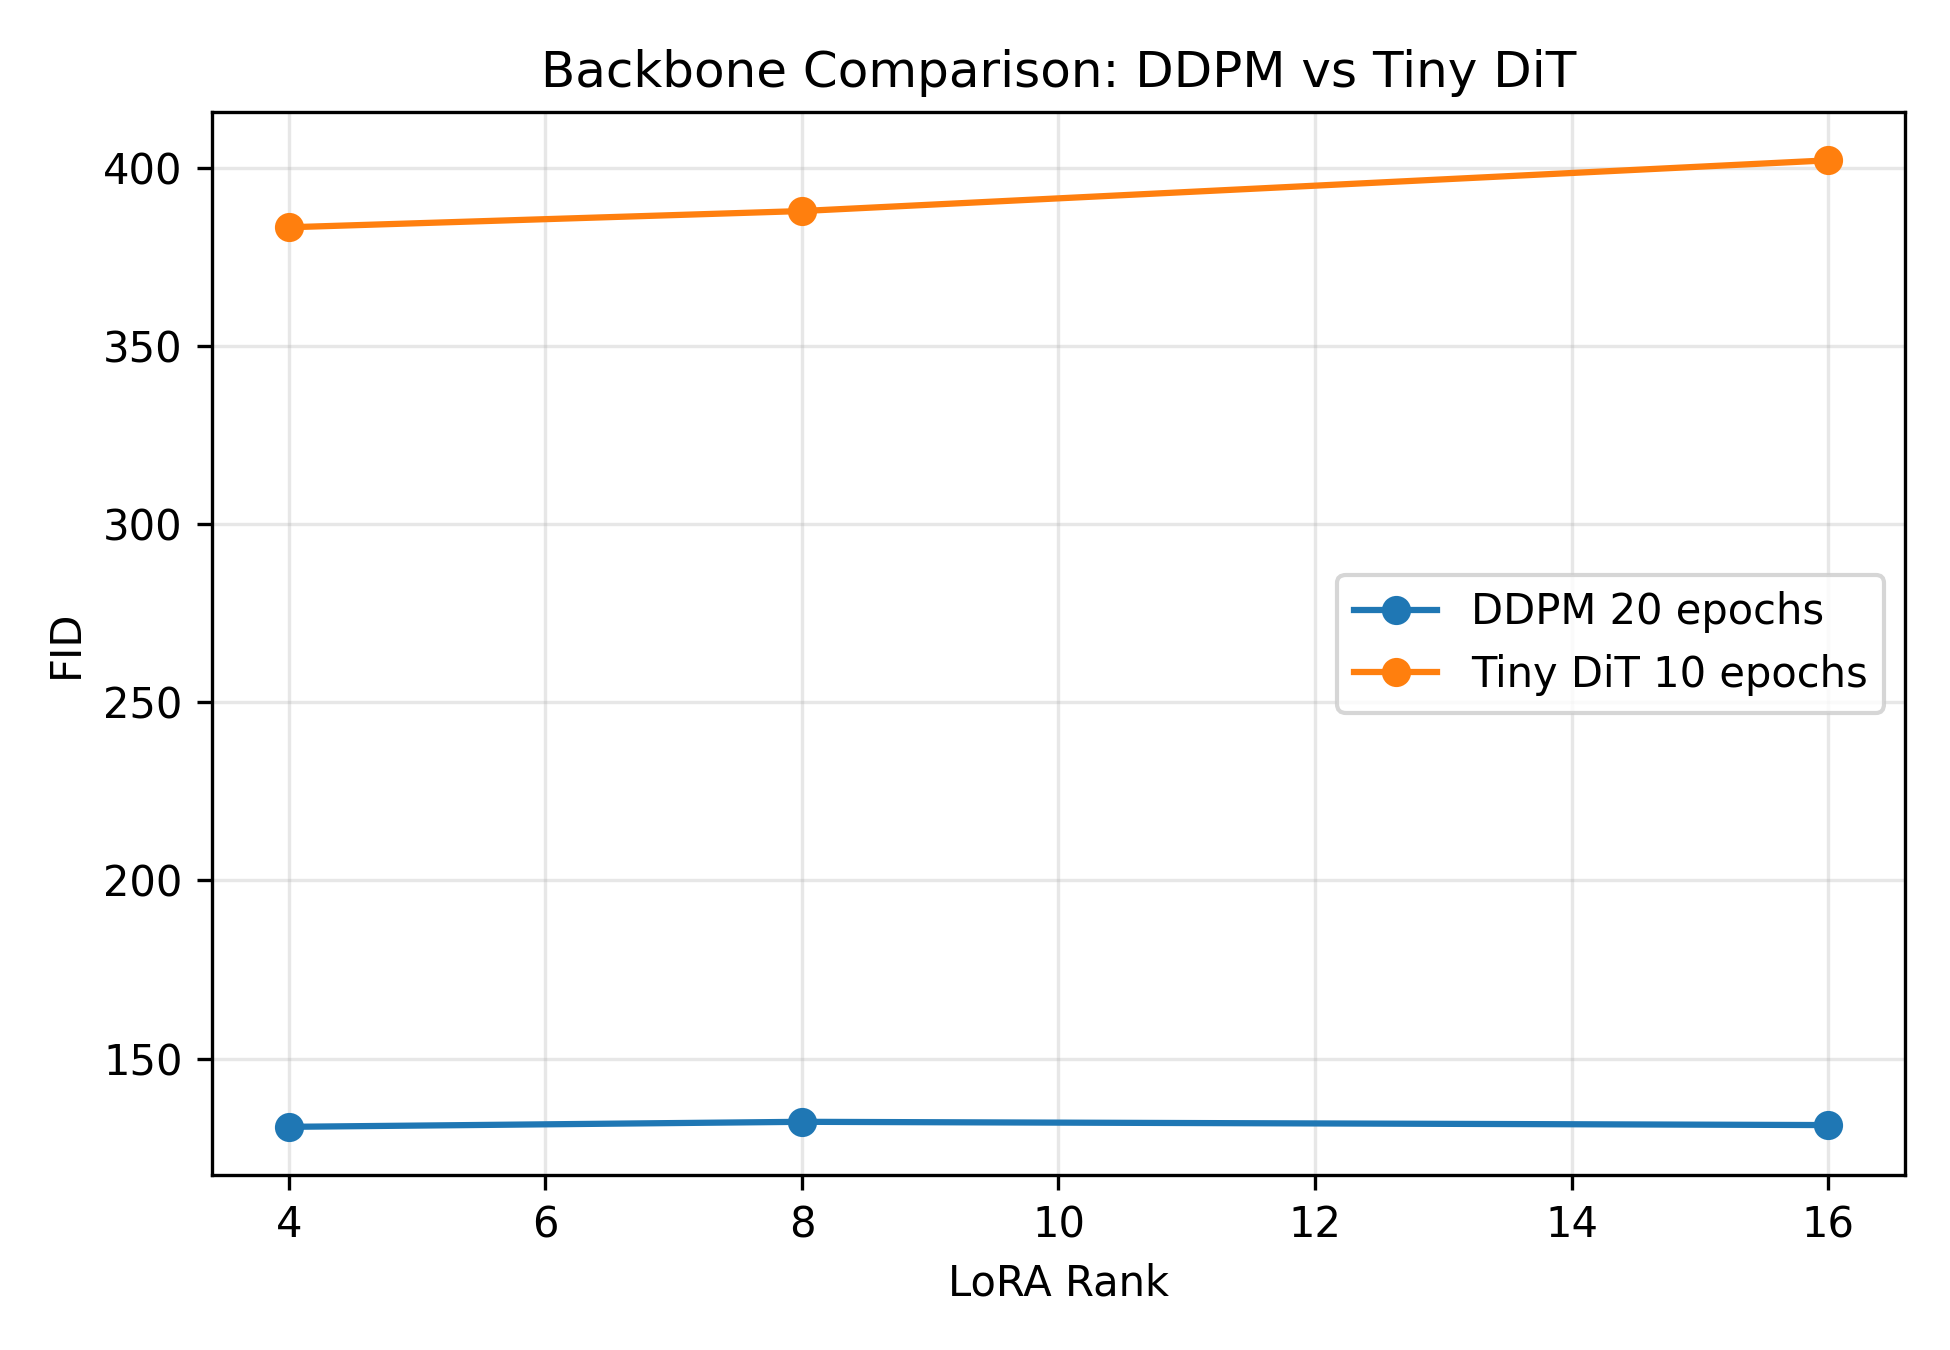
\includegraphics[width=0.9\linewidth]{../outputs/figures/ddpm_vs_tiny_dit_fid_rank4_8_16.png}
  \caption{Backbone comparison: DDPM (20 epochs) vs. Tiny DiT (10 epochs) for ranks 4, 8, and 16.}
  \label{fig:ddpm_vs_tiny}
\end{figure}

Absolute FID levels are not directly comparable across backbones as quality baselines differ; the key result is trend consistency in rank ordering under controlled settings.
